\documentclass{article}
\usepackage{tikz}

\begin{document}

% Title and author information
\title{My Document}
\author{Your Name}
\date{\today}

\maketitle
\centering
% TikZ picture of pendulum on cart
\begin{tikzpicture}
    % Pendulum
    \draw (0,0) node[circle, fill=black, inner sep=0pt, minimum size=3pt] {};
    \draw (0,0) node[left] {$O$};
    \draw (-30:4) node[circle, fill=black, inner sep=0pt, minimum size=3pt] {};
    \draw (-30:8) node[circle, fill=black, inner sep=0pt, minimum size=3pt] {};
    \draw (0,0) -- (-30:4) node[midway, above right] {$r$};
    \draw (0,0) -- (-30:8) node[midway, above right] {$L$};

    % mg
    \draw[->] (-30:4) -- ++(0,-1) node[right] {$mg$};

    % n-t
    \draw[->] (0,0) -- (150:2) node[below] {$n$};
    \draw[->] (0,0) -- (60:2) node[below] {$t$};

    % Theta
    \draw[dotted] (0,0) -- (0,-4);
    \draw (-90:1) arc (-90:-30:1) node[midway, below] {$\theta$};

    % x-axis
    \draw (5,0.2) -- (5,-0.2);
    \draw[->] (5,0) -- (6,0) node[right] {$x$};
\end{tikzpicture}

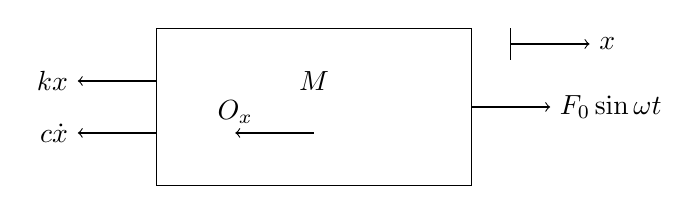
\begin{tikzpicture}
    % Cart
    \draw (-2,0) rectangle (2,2);
    \draw (0, 1.33) node {$M$};

    % Pendulum Force
    \draw[->] (0,0.67) -- (-1,0.67) node[above] {$O_x$};

    % Damper and Sprint
    \draw[->] (-2,0.67) -- (-3,0.67) node[left] {$c\dot x$};
    \draw[->] (-2,1.33) -- (-3,1.33) node[left] {$kx$};

    % Forcing term
    \draw[->] (2,1) -- (3,1) node[right] {$F_0\sin\omega t$};

    % x-axis
    \draw (2.5,2) -- (2.5,1.6);
    \draw[->] (2.5,1.8) -- (3.5,1.8) node[right] {$x$};
\end{tikzpicture}

\end{document}